% ============================================================
% CHƯƠNG 7: KẾT QUẢ & ĐÁNH GIÁ
% ============================================================
\chapter{Kết quả và đánh giá}
\label{ch:results}

\section{Tổng hợp kết quả huấn luyện}
\label{sec:results_training}

\begin{table}[H]
    \centering
    \caption{Tổng hợp kết quả huấn luyện các phiên bản YOLO26}
    \label{tab:results_summary}
    \begin{tabular}{lrrr}
        \toprule
        \textbf{Phiên bản}     & \textbf{Epochs} & \textbf{mAP50} & \textbf{mAP50-95} \\
        \midrule
        YOLO26 gốc Ultralytics & 100             & \textbf{0.809} & \textbf{0.593}    \\
        YOLO26 Custom last run & 100             & \textbf{0.778} & ---               \\
        \bottomrule
    \end{tabular}
\end{table}

Phiên bản YOLO26 Custom last run đạt kết quả mAP50 = 0.778 ở epoch 100, tiệm cận hiệu năng của phiên bản gốc (0.809) nhưng được tối ưu hóa tốt hơn cho suy luận thời gian thực.

\begin{figure}[H]
    \centering
    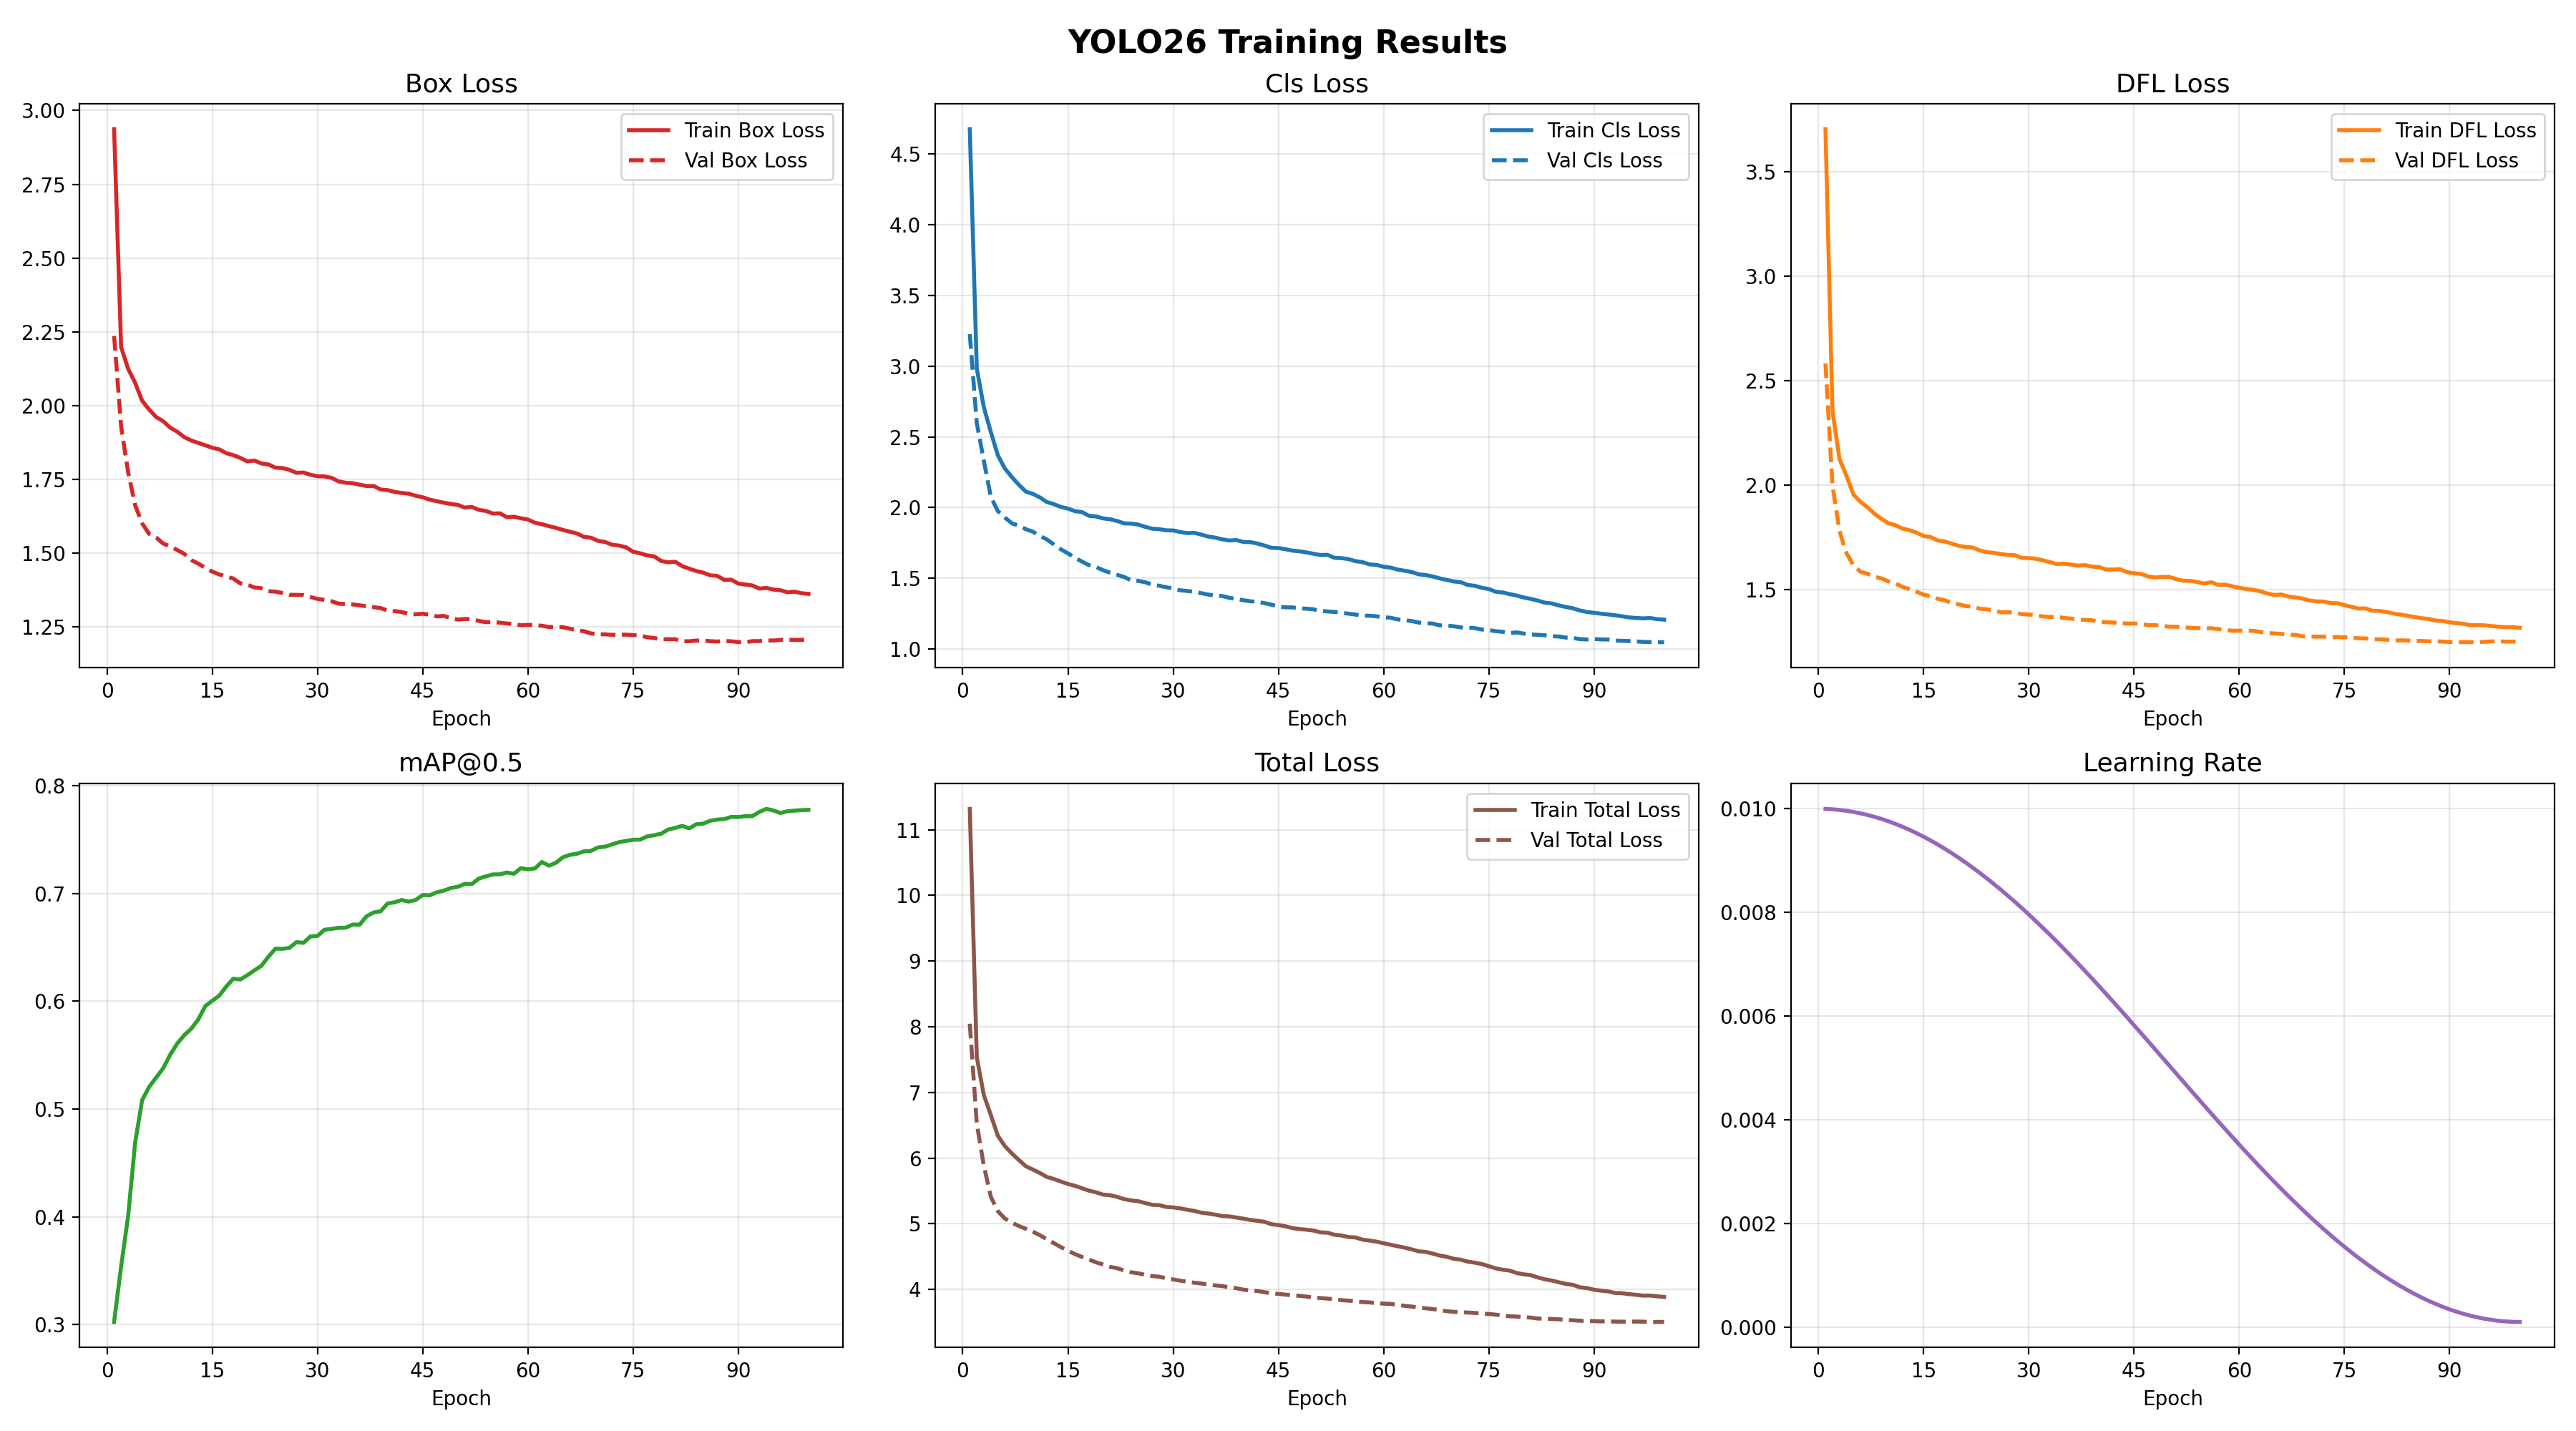
\includegraphics[width=\textwidth]{figures/custom_results.png}
    \caption{Biểu đồ các đường loss và chỉ số đánh giá (metrics) trong quá trình huấn luyện YOLO26 Custom last run qua 100 epochs.}
    \label{fig:results_plot}
\end{figure}

\begin{figure}[H]
    \centering
    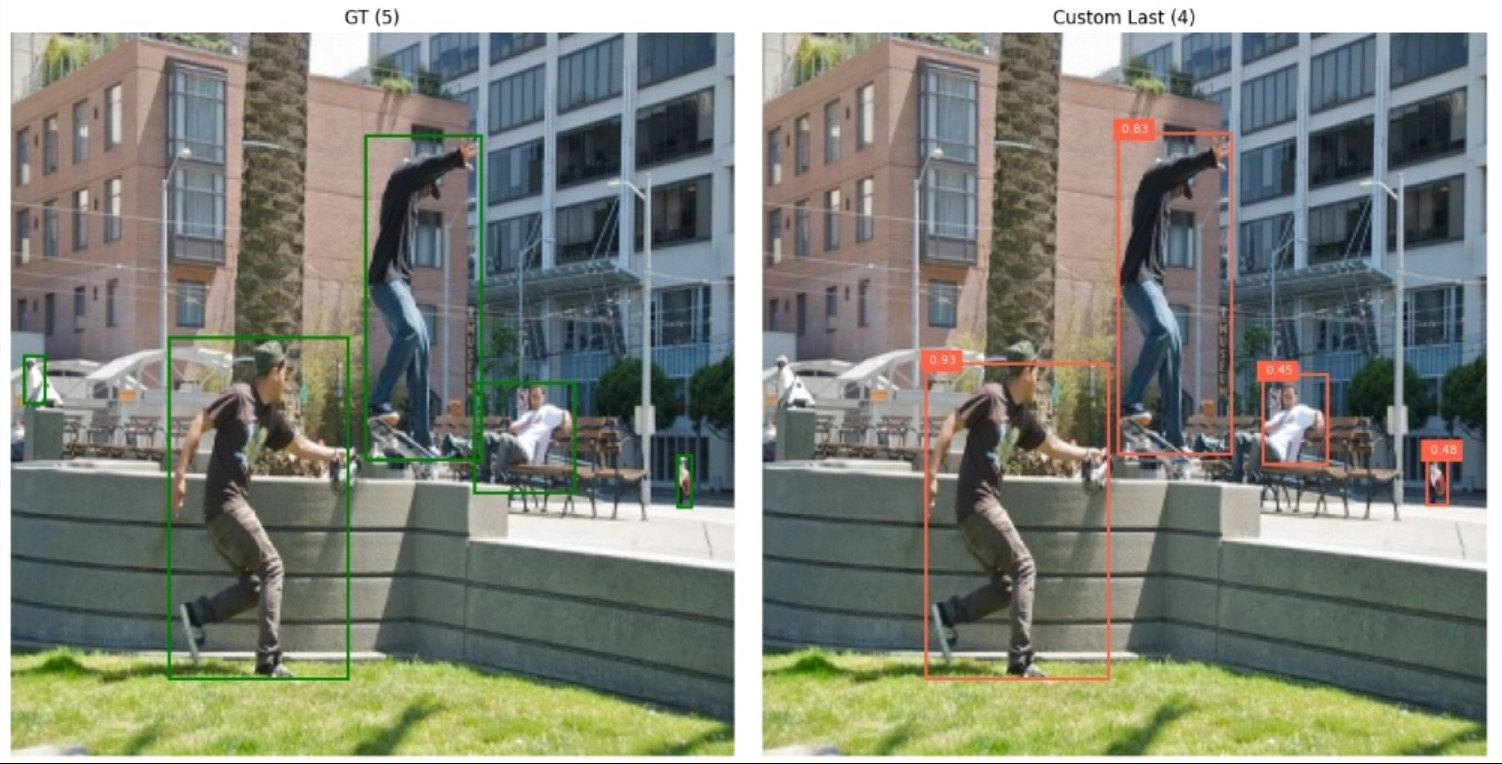
\includegraphics[width=0.95\textwidth]{figures/infimg.jpg}
    \caption{Hình ảnh so sánh kết quả nhận diện thực tế giữa Ground Truth GT và mô hình YOLO26 Custom last run.}
    \label{fig:pred_images}
\end{figure}

\section{Kết quả inference trên Raspberry Pi 5}
\label{sec:results_inference}

Để đánh giá khả năng hoạt động thực tế của mô hình trên các thiết bị phần cứng giới hạn, nhóm nghiên cứu đã triển khai mô hình \yolo định dạng NCNN trên bo mạch \rpi phiên bản 4GB RAM (CPU Broadcom BCM2712 Quad-core ARM Cortex-A76 @ 2.4GHz), chạy hệ điều hành Raspberry Pi OS (headless mode, tắt hoàn toàn giao diện đồ họa GUI).

Kết quả sơ bộ cho thấy \yolo NCNN đạt tốc độ detection-only $\sim$45 FPS\footnote{Con số cần được xác minh lại trong các thí nghiệm tiếp theo.} ở độ phân giải 320$\times$320 trên \rpi 4GB mà không cần bộ tăng tốc AI.

Thực nghiệm thu được cho thấy hiệu năng suy luận (inference speed) cực kỳ ấn tượng của mô hình \yolo NCNN khi so sánh trực tiếp với YOLOv8 NCNN ở các độ phân giải đầu vào khác nhau, chi tiết như sau:

\begin{itemize}
    \item \textbf{Độ phân giải $320 \times 320$}: Mô hình \yolo NCNN đạt tốc độ xử lý trung bình \textbf{45,61 FPS} (tương đương khoảng 21,92 ms/khung hình), nhanh hơn so với YOLOv8 NCNN đạt 44,36 FPS. Tốc độ này đáp ứng hoàn hảo yêu cầu xử lý thời gian thực (real-time) đối với các hệ thống camera bám vết.
    \item \textbf{Độ phân giải $480 \times 480$}: Tốc độ xử lý của mô hình đạt \textbf{26,67 FPS} (khoảng 37,50 ms/khung hình) so với YOLOv8 NCNN đạt 25,26 FPS, vẫn đảm bảo tính liên tục cao của luồng video.
    \item \textbf{Độ phân giải $640 \times 640$}: Mô hình đạt tốc độ \textbf{15,09 FPS} (khoảng 66,27 ms/khung hình) so với YOLOv8 NCNN đạt 13,90 FPS.
\end{itemize}

Hiệu năng ấn tượng này đạt được là nhờ sự kết hợp giữa kiến trúc \yolo được tối ưu hóa sâu (thiết kế tinh giản, đặc trưng Direct Regression không sử dụng phân phối khoảng cách phức tạp như các dòng YOLO khác) và cơ chế \textbf{NMS-free} (Direct Regression / One-to-One Head). Khác với các mô hình truyền thống phải thực hiện thuật toán Non-Maximum Suppression (NMS) trên CPU thiết bị biên để lọc trùng bounding box gây nghẽn cổ chai hiệu năng, \yolo suy luận trực tiếp ra tọa độ hộp bao tối ưu cho mỗi đối tượng.

Cụ thể, tổng thời gian suy luận 21,92 ms cho mỗi khung hình ở độ phân giải $320 \times 320$ được phân rã như sau:
\begin{itemize}
    \item \textbf{Tiền xử lý (Preprocessing)}: Mất khoảng \textbf{1,5 ms} cho các thao tác chuẩn hóa ảnh đầu vào và chuyển đổi định dạng ma trận NCNN.
    \item \textbf{Suy luận mô hình (Inference)}: Mất khoảng \textbf{19,5 ms} cho quá trình lan truyền xuôi (forward pass) qua mạng nơ-ron trên CPU.
    \item \textbf{Hậu xử lý (Postprocessing)}: Chỉ mất khoảng \textbf{0,9 ms} để giải mã tọa độ hộp bao trực tiếp mà không cần chạy NMS.
\end{itemize}

Biểu đồ so sánh chi tiết tốc độ xử lý giữa hai mô hình được thể hiện ở \figref{fig:fps_benchmark_results}.

\begin{figure}[H]
    \centering
    
\includegraphics[width=0.85\textwidth]{fps_benchmark.png}
    \caption{Biểu đồ so sánh tốc độ xử lý (FPS) giữa YOLO26 NCNN và YOLOv8 NCNN trên Raspberry Pi 5 ở các độ phân giải 320, 480 và 640.}
    \label{fig:fps_benchmark_results}
\end{figure}

Để đánh giá hiệu năng benchmark chi tiết hơn về mặt tài nguyên và thời gian suy luận (inference speed) thực tế, nhóm đã tiến hành đo đạc hiệu năng của mô hình YOLO26 gốc (\texttt{y262.pt}) so với phiên bản YOLO26 Custom sau tối ưu hóa (\texttt{yolo26n\_lite.pt}). Kết quả so sánh benchmark được tổng hợp trong Bảng~\ref{tab:benchmark_custom_vs_original}.

\begin{table}[H]
    \centering
    \caption{Bảng so sánh hiệu năng benchmark giữa YOLO26 gốc và YOLO26 Custom}
    \label{tab:benchmark_custom_vs_original}
    \begin{tabular}{lrr}
        \toprule
        \textbf{Thông số}                         & \textbf{Original YOLO26} & \textbf{Custom YOLO26}     \\
        \midrule
        Kích thước mô hình (Model Size)           & 5.10 MB                  & 5.60 MB\textsuperscript{*} \\
        Số lượng tham số (Parameters)             & 2.504 M                  & 3.986 M                    \\
        Lượng tính toán (GFLOPs @ 320$\times$320) & 0.721                    & 2.335                      \\
        Thời gian suy luận (Inference Speed)      & 69.86 ms                 & 96.98 ms                   \\
        \bottomrule
    \end{tabular}

    \vspace{4pt}
    \small\textsuperscript{*} Kích thước mô hình Custom sau khi loại bỏ O2M head (định dạng FP16). Kích thước phiên bản FP32 đầy đủ là 6.20 MB.
\end{table}

\textbf{Nhận xét}:
\begin{itemize}
    \item Phiên bản YOLO26 Custom có kích thước mô hình (5.60 MB) và số lượng tham số lớn hơn (3.986 M so với 2.504 M).
    \item Lượng tính toán (GFLOPs) của phiên bản Custom đạt 2.335 GFLOPs ở độ phân giải 320$\times$320, cao hơn đáng kể so với phiên bản gốc (0.721 GFLOPs).
    \item Do lượng tính toán tăng lên, thời gian suy luận (Inference Speed) trên CPU của Raspberry Pi 5 tăng từ 69.86 ms lên 96.98 ms, tương ứng với mức giảm FPS nhẹ, phải xem lại model custom trong thời gian tới.
\end{itemize}

\section{Đánh giá}
\label{sec:results_evaluation}

\subsection{Những gì đã làm được}

\begin{enumerate}[label=\arabic*)]
    \item \textbf{Nghiên cứu kiến trúc}: Nhóm đã nghiên cứu và trình bày chi tiết toàn bộ kiến trúc \yolo, từ Backbone đến Detection Head, bao gồm cả các cơ chế huấn luyện tiên tiến (ProgLoss, MuSGD, STAL).

    \item \textbf{Custom implementation}: Xây dựng thành công \yolo từ đầu (from scratch) bằng PyTorch thuần, đạt mAP50 = 0.778 sau 100 epochs --- chứng minh sự hiểu biết sâu về kiến trúc.

    \item \textbf{Triển khai edge}: Demo thành công detection trên \rpi 4GB không cần accelerator, với pipeline triển khai đơn giản (NCNN).

    \item \textbf{Dataset}: Xây dựng bộ dữ liệu COCO Person 320 gồm 49.811 ảnh huấn luyện, lớn hơn đáng kể so với khóa trước (2.207 ảnh).
\end{enumerate}

\subsection{Hạn chế}

\begin{enumerate}[label=\arabic*)]
    \item Mô hình custom cần tiếp tục tinh chỉnh hyperparameters để tối ưu hóa thêm hiệu năng.
    \item Cần xác minh lại con số FPS benchmark.
    \item Nếu được cần tiếp tục sửa đổi và kiểm tra lỗi sai để cải thiện kết quả của mô hình custom so với mô hình gốc.
\end{enumerate}

\section{Hướng phát triển}
\label{sec:results_future}

\subsection{Đồ án 2 (dự kiến)}

\begin{itemize}
    \item Tích hợp ByteTrack~\cite{bytetrack} để tracking diễn giả liên tục.
    \item Hoàn thiện custom \yolo và triển khai trên \rpi.
    \item Thiết kế hệ thống điều khiển servo Pan-Tilt cơ bản.
\end{itemize}

\subsection{Khóa luận tốt nghiệp (dự kiến)}

\begin{itemize}
    \item Hoàn thiện toàn bộ pipeline: detection $\to$ tracking $\to$ PID servo control.
    \item Xây dựng giao diện giám sát và điều khiển.
    \item Truyền dẫn video thời gian thực qua mạng.
    \item Tối ưu hóa mô hình cho các điều kiện ánh sáng và bối cảnh đa dạng.
\end{itemize}
